\section{User Interaction}
\fixme{Name change}
\label{sec:interaction}
The user interacts with \projectname{} through \deno{B}.
\at{1} and \at{2} requires that the user must be granted access to the system before being able to interact with it.
This access is granted through a valid login and privileges.
When \deno{B} initiates a connection to \deno{M}, it returns a login view.
This is done by the access controller, which is described in Figure~\ref{tab:access_controller_actions} in Appendix~\ref{app:controller_actions}.
The user enters his login credentials in the login view and \deno{B} sends a login request to \deno{M}.
Following a successful login the user is redirected to the drone view, where the user is shown a menu and the available drones. \\
% Following a successful login the users credentials is stored on \deno{B} as described in Section~\ref{sec:design_client}.

\deno{B} can then interact with any of the models described in Section~\ref{section:uml_notation} that have associated views.
The general interaction with these models is similar, and the interaction with drones is described as an example.
When \deno{B} requests to interact with drones, the drone controller returns a view containing a list of all drones available to the user.
This list contains all drones the user has access to based on his privileges.
The users privileges are retrieved through the users model.
For each drone in the system it is checked if the user has privileges that grants him access to the drone.
From the drones list the user can edit a drone, or delete a drone.
Drones are added automatically to the system through the initialization messages send by the \deno{Slaves}.
To make a drone usable in \projectname{}, it must be added to a company as reflected in the object model, see Section~\ref{subsec:objects}. \\

\begin{figure}[htb]
    \centering
    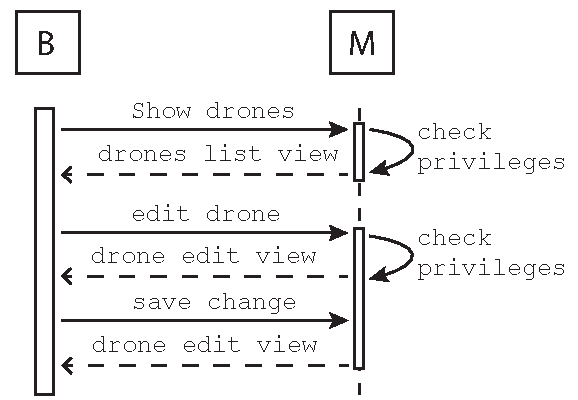
\includegraphics[width=\textwidth]{gfx/interaction_sequence_diagram.pdf}
    \caption{Illustration interaction between \deno{B} and \deno{M}.}
    \label{fig:interaction_sequence}
\end{figure}

The process of editing a drone is illustrated in Figure~\ref{fig:interaction_sequence}.
\deno{B} request the list of drones from \deno{M}, and is returned a list of drones based on his privileges.
\deno{B} then requests to edit a drone and \deno{M} ensures the user has needed privilege to edit the drone.
If this is the case, \deno{B} receives a view from \deno{M} where the user can input data to update the drone with.
The user can then choose save the entered data and \deno{B} then sends it to \deno{M} which saves them in the \deno{DB}.
\deno{M} then returns \deno{B} an updated edit view the drone.

As mentioned a user deletes a drone through the drones list send to \deno{B} by \deno{M}.
When a delete request is send from \deno{B} to \deno{M} for a drone, \deno{M} deletes all links the drone has with other object in \deno{DB}.
The drone is not deleted from the system, as described in Section~\ref{subsec:objects}\fxfatal{Dette skal skrives hvis det ikke kommer til at st� i object model}.

Some of the views require asynchronous behaviour, that allows the views to be updated without recomputing it.
As an example when editing the current view can be updated asynchronously insted of having \deno{M} recompute it.
In this way some of the computation is moved from \deno{M} to \deno{B}, as described in Section~\ref{sec:design_client}.
\fxfatal{User eller \deno{B} n�r vi snakker om brugeren}

From the drones' list \deno{B} can request to pilot or view of the drones' listed.
When \deno{B} requests to pilot a drone the process of retrieving a session key from the drones' associated \deno{S} is initiated by the drones controller.
\deno{B} is redirected to a page containing the video player described in Section~\ref{sec:design_client} when the session key is recieved.
From this page \deno{B} can view the drones video feed and send control commands to the drone as described in Sections~\ref{sec:design_client} and \ref{sec:design_slave}.


%Login -> access i systemet, noget med privileges
%Interaction with